\chapter{DATA C100: Introduction to Modeling and Linear Regression}

\section{Motivation}
A \textbf{model} is an idealized representation of a system, which are mostly mathematical. Their mathematical properties lend us the computational opportunity to abstract a system in a computational space! \\
In general, the machine learning works we perform in DATA C100 lend strength from constructions of models that allow us to predict new values from old data.

Outside the context of machine learning, there are a few categories of models that human history has used:
\begin{bindenum}
    \item \textbf{Deterministic Physical (Mechanical) Models}, such as kinematics equations.
    \item \textbf{Probabilistic Models}, which models how random processes can evolve.
    \item \textbf{Statistical Models}, which associates variables via statistical analysis.
    \item \textbf{Informal Models}, which are essentially stories or human-understandable descriptions of a complex phenomenon. Many pictographics might be an informal model.
\end{bindenum}
The introduction towards several categories of models only reinforce the idea that it is used for understanding the world as a complex phenomenon as well as providing predictions towards unseen cases.

Quite frequently, we would like to create models that are simple and interpretable, when we attempt to understand the association between different variables.
But when we attempt to make extremely accurate preditcions, we would also risk providing an uninterpretable model whose complexity supports its performance. \\
Both directions of modeling in terms of interpretability have been used, and made their successes in each of their mission. Notably, complex models occur a lot in deep learning. \\

\section{A Demonstration: Simple Linear Regression}

\subsection{What is a Regression Line?}
Suppose we have a crowd of data points spread across a 2D plot, which we call a scatterplot, and we want to predict one dimension of the data point from another, then we may use a regression line:
\begin{ln-define}{Regression Line}{}
    A \textbf{Regression Line} is a linear model that attempts to predict a feature of a specific data-point via a linear combination of other features.
    \tcblower
    \begin{center}
        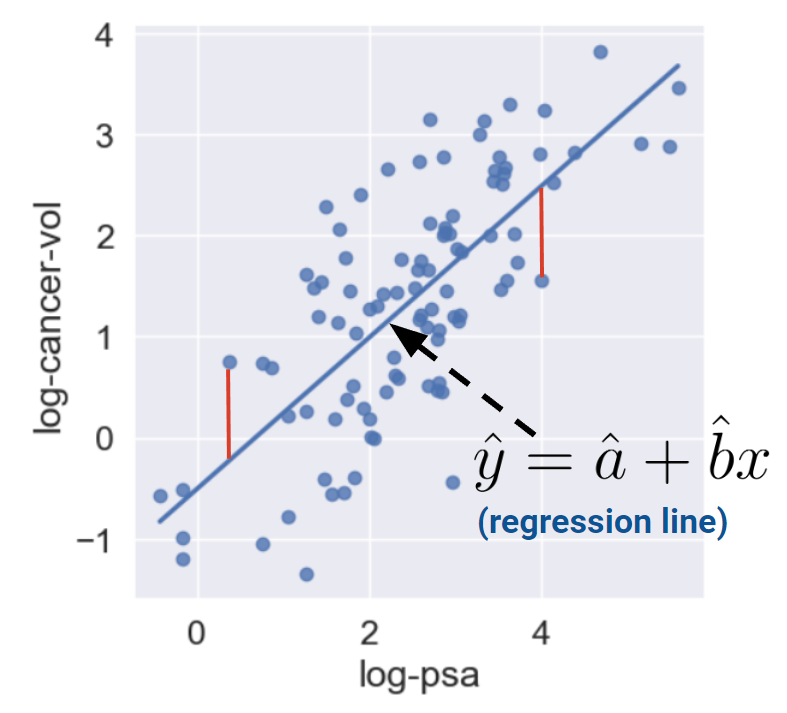
\includegraphics[scale=0.4]{figs/ln01/regression-line.png}
    \end{center}
\end{ln-define}
For now, let us simplify our description: ``We would like to predict $y$ by $x$''. Then the way we predict is by assuming there is a coefficient $a$ and $b$ such that:
\[y = a + bx\]
would accurately predict $y$ for any provided $x$. \\
The most accurate parameter of this line would be denoted as $\hat{a}$ and $\hat{b}$, and the prediction following these best parameters would be denoted as $\hat{y}$, hence the regression line equation:
\[\hat{y} = \hat{a} + \hat{b}x\]

In summary, the hat symbol $\hat{x}$ stands for an estimation of the original value of parameter $x$. \\
Let us expound on what is happening here. \\
Sometimes, the real values $a$, $b$ of a regression line is not solvable. These parameters assume a 100\% accuracy for the predictions they offer, while in an extremeley wide majority of realistic conditions, 100\% accuracy is impossible.
Therefore, we instead look for some estimated values of these parameters that we expect to close the prediction error between the line with $a, b$ and the line with estimated parameters $\hat{a}, \hat{b}$.

Now, each dataset that we attempt to apply a regression line onto has a specific statistic called \textbf{correlation}:
\begin{ln-define}{Pearson's Correlation Coeffcient}{}
    A \textbf{correlation} (denoted as $r$), formally known as the ``Pearson's Correlation Coeffcient'', quantifies how linearly associated two variables $x$ and $y$ may be via the following formula:
    \[
        r = \frac{1}{n} \sum_{i = 1}^n \bigg( \frac{x_i - \overline{x}}{\sigma_x} \bigg) \bigg( \frac{y_i - \overline{y}}{\sigma_y} \bigg)
    \]
    In other words, this is the average of the product of $x$ and $y$, both measured in standard units.
    \begin{center}
        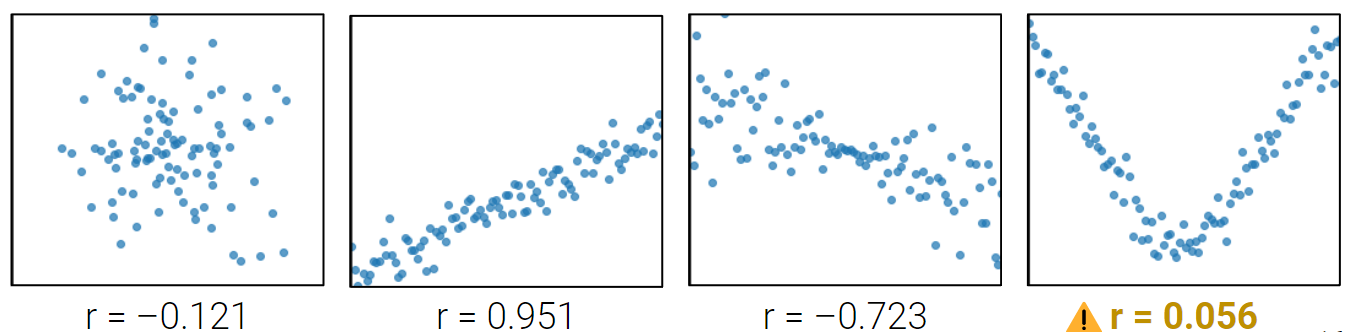
\includegraphics[scale=0.4]{figs/ln01/linear-correlation.png}
    \end{center}
\end{ln-define}

At this point, you will probably have the following concerns:
\begin{bindenum}
    \item What does it mean when a parameter is ``best'' or ``most accurate''?
    \item How do we obtain such parameters?
\end{bindenum}
And here is where we deal with the mathematics of regression lines.

\subsection{Model Selection: Simple Linear Regression}
The \textbf{Simple Linear Regression} model is a model using the regression line to predict the $y$ of a datapoint for the $x$ of a datapoint. \\
In most definitions, Simple Linear Regression is bound to only produce a two-dimensional regression line.

Such a model's prediction relies entirely on the value of its parameters. We recognize this by saying that Simple Linear Regression is a \textbf{parametric model}, described by its parameters $a$ and $b$.

Once again, you might have noticed from the few graphs above that, the regression line doesn't accurately predict every single point. It is born from a set of points that don't necessarily form a line. Therefore, the best parameters that we provide it (an estimation, denoted $\hat{a}$ and $\hat{b}$), are what we call the sample-based estimate of the inexistent, completely correct regression line. \\
Following that same logic, we noted the result of prediction as $\hat{y}$: our best estimate of the actual $y$ of a new, unseen datapoint.

\subsection{Quantifying Errors: Loss Functions}
To quantify how ``good'' a prediction is, we would like to use a loss function, which characterizes the net error on a set of datapoints:
\begin{ln-define}{Loss Function}{}
    A \textbf{loss function} is a function that characterizes the cost in predictions for choosing a set of parameters. \\
    It quantifies how bad a prediction is for a single observation. The closer our prediction is to the actual observed value, the better the prediction, therefore, the lower the loss. Vice versa.
\end{ln-define}
The choice of loss function affcets how we customize our model to adapt to mistakes. While it affects the accuracy of estimations, it would also decide the computational cost of estimation, as some loss functions are very costly to calculate for computers. \\
For Simple Linear Regression, we usually bother with two choices of loss functions:
\begin{ln-define}[sidebyside]{Loss Functions of SLR}{}
    \textbf{Squared Loss} (L2 Loss) \\
    \[L(y, \hat{y}) = {(y - \hat{y})}^2\]
    This is a reasonable choice because there would be no loss when prediction is equal to observed value, and provide a lot of loss for predictions that are far from the observed values.
    \tcblower
    \textbf{Absolute Loss} (L1 Loss) \\
    \[L(y, \hat{y}) = |y - \hat{y}|\]
    This is a reasonable choice because there would be no loss when prediction is equal to observed value, and provide a fair amount of loss at a uniform sign (positive) for predictions that are far from the observed values (benefited from the absolute value).
\end{ln-define}
Since we concern how costly our model's predictions are for the entire data set, the natural measure of how good a model is would be the average loss of model across all data points. This is also known as \textbf{empirical risk}:
\begin{ln-define}{Empirical Risk}{}
    The empirical risk is the average loss of a model across all data points. \\
    Minimizing empirical risk provides the optimal estimated parameters of a model for the corresponding loss function. \\
    Mathematically expressed,
    \[\hat{R}(\theta) = \frac{1}{n} \sum_i L(y_i, \hat{y}_i)\]
    Here, $\theta$ represents the parameters of the model.
\end{ln-define}
Now, let us inspect the case where we attempt to minimize the empirical risk with our loss being L2 loss function. In this case, we call our empirical risk \textbf{Mean Squared Error}.
\begin{ln-derive}{Estimated Intercept of Simple Linear Regression under MSE}{}
    To recall:
    \[MSE(a, b) = \frac{1}{n} \sum_i {(y_i - a - b x_i)}^2\]
    To minimize this function, we will find the conditions where the partial derivative of $MSE$ with respect to every parameter is $0$. \\
    \textbf{Minimizing a}: \\
    \begin{align*}
        \pdv{MSE}{a} &= \frac{1}{n} \times \sum_i 2\frac{\delta}{\delta a}(y_i - a - b x_i)(y_i - a - b x_i) \\
        &= \frac{1}{n} \times \sum_i -2(y_i - a - b x_i) \\
        &= -\frac{2}{n} \sum_i (y_i - a - b x_i) \\
        \frac{1}{n} \sum_i (y_i - \hat{y}_i) &= 0 \\
        \sum_i (y_i - a - b x_i)
        &= \sum_i (y_i) - a - b\sum_i (x_i) \\
        &= \overline{y} - a - b \overline{x} = 0 \\
        a &= \overline{y} - b \overline{x}
    \end{align*}
\end{ln-derive}
And before moving onto the next derivation, let us pay attention to an interesting property about the error between one observed value $y_i$ and one predicted value $\hat{y_i}$. \\
First of all, this value is called a ``\textbf{residual}'', standing for the error of prediction written in the direction of $y_i - \hat{y_i}$. \\
Second of all, an optimal regression line, according to our derivation above, would have the property of:
\[\frac{1}{n} \sum_i (y_i - \hat{y}_i) = 0\]
The sum of residuals across all datapoints is $0$, and consequentially, the mean of residuals across all datapoints is also $0$.
\begin{ln-derive}{Estimated Slope of Simple Linear Regression under MSE}{}
    \textbf{Minimizing b}: \\
    \begin{align*}
        \pdv{MSE}{b} &= \frac{1}{n} \times \sum_i 2\frac{\delta}{\delta b}(y_i - a - b x_i)(y_i - a - b x_i) \\
        &= \frac{1}{n} \times \sum_i -2x_i(y_i - a - b x_i) \\
        &= -\frac{2}{n} \sum_i x_i(y_i - a - b x_i) \\
        \frac{1}{n} \sum_i x_i(y_i - \hat{y}_i) &= 0 \\
        \frac{1}{n} \sum_i x_i(y_i - \hat{y}_i) - \frac{1}{n} \sum_i \overline{x} (y_i - \hat{y}_i)
        &= \frac{1}{n} \sum_i (x_i - \overline{x}) (y_i - \hat{y}_i) \\
        &= \frac{1}{n} \sum_i (x_i - \overline{x}) (y_i - \overline{y} - b(x_i - \overline{x})) = 0 \\
        \frac{1}{n} \sum_i (x_i - \overline{x}) (y_i - \overline{y})
        &= b \frac{1}{n} \sum_i (x_i - \overline{x}) (x_i - \overline{x}) \\
        r_{x, y} \sigma_x \sigma_y &= b \sigma_x^2 \\
        b = r \frac{\sigma_y}{\sigma_x}
    \end{align*}
    \tcblower
    Conclusion:
    \[
        \begin{cases}
            \hat{a} = \overline{y} - \hat{b} \overline{x} \\
            \hat{b} = r \frac{\sigma_y}{\sigma_x}
        \end{cases}
    \]
\end{ln-derive}
So at last, we also find that the optimizing condition of SLR model would be:
\[
    \begin{cases}
        \frac{1}{n} \sum_i (y_i - \hat{y}_i) &= 0 \\
        \frac{1}{n} \sum_i x_i(y_i - \hat{y}_i) &= 0
    \end{cases}
\]
Which can be interpreted respectively as that, in an optimal regression line:
\begin{bindenum}
    \item The residuals average to 0.
    \item As a vector, the residuals are orthogonal to the predictor variable.
\end{bindenum}
